\chapter{Evaluación experimental}
\label{cap:evaluacionexperimental}

En el presente capítulo se presenta los resultados obtenidos de las diferentes implementaciones para los métodos propuestos en la secciones anteriores. Se comienza por la implementación de los diferentes enfoques de los métodos de procesamiento de transacciones de lectura, posteriormente se muestra los resultados obtenidos para los diferentes métodos de predicción de tiempos de respuestas para consultas y el comportamiento que tienen para diferente conjunto de datos. Finalmente se presenta el comportamiento de las diferentes estrategias de planificación presentadas para diferentes tipos de escenarios.


\section{Hardware y conjunto de datos}
\label{evaluacionexperimental:hardwareydatos}
%% Hablar un poco del hardware utilizado en los experimentos

Se utilizaron dos conjuntos de datos para llevar a cabo los experimentos, estos son frecuentemente usados por la comunidad del área de Information Retrieval para experimentar. El primero de ellos es GOV2, este conjunto es una colección de aproximadamente 25 millones de páginas Web obtenida desde los dominios .gov y que pesa 426 GB. La otra colección de datos utilizada es la ClueWeb09, la cual fue creada para apoyar la investigación en recuperación de la información y las tecnologías relacioanadas con el lenguaje humano. Consiste en alrededor de un billón de páginas en diez lenguajes diferentes y 50 millones en Inglés. ClueWeb09 pesa 5 TB en forma comprimidad y 25 TB descomprimida. 

% Las consultas (queries)



\section{Wand multithreaded}
\label{evaluacionexperimental:wm}
En esta sección se muestra la implementación de dos enfoques para el procesamiento de consultas a través del algoritmo Wand \citep{Broder:2003}. El primer enfoque es el esquema de heap locales (LH), en el que cada thread obtiene sus mejores documentos para una query dada y luego una hebra maestra se encarga de mezclar todos los resultados de cada uno de los threads para construir en conjunto top-K final; el segundo enfoque es el enfoque de heap compartido (SH), en el que se tiene un heap visible a todos lo shilos de ejecución y en donde ellos compiten por el acceso a esta estructura de datos. El detalle del diseño de los enfoques LH y SH están disponibles en \ref{scheduling:wlh} y \ref{scheduling:whc}. 

\subsection{Esquema LH}
\label{evaluacionexperimental:esquemalh}

\begin{figure}[th!]
\centering
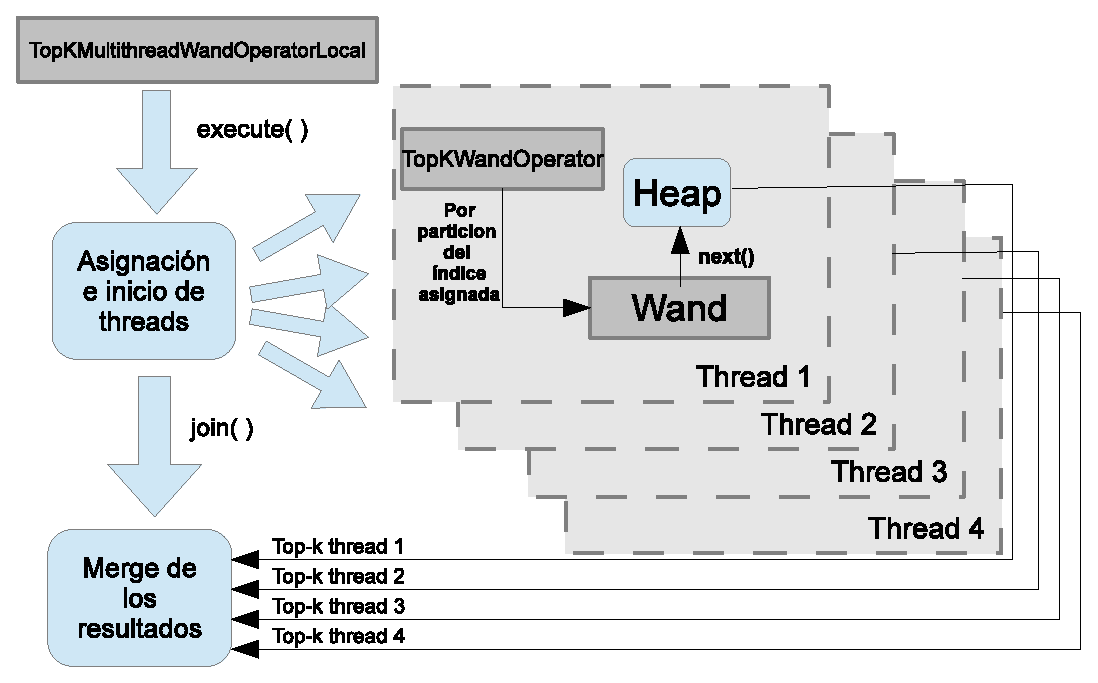
\includegraphics[scale=.75]{images/ejecucion_topkmultithreadwandopLOCAL.eps}
\caption{Esquema de ejecución enfoque LH}
\label{fig:esquema_ejecucion_wandlh}
\end{figure}



\subsection{Esquema SH}
\label{evaluacionexperimental:esquemash}

\begin{figure}[th!]
\centering
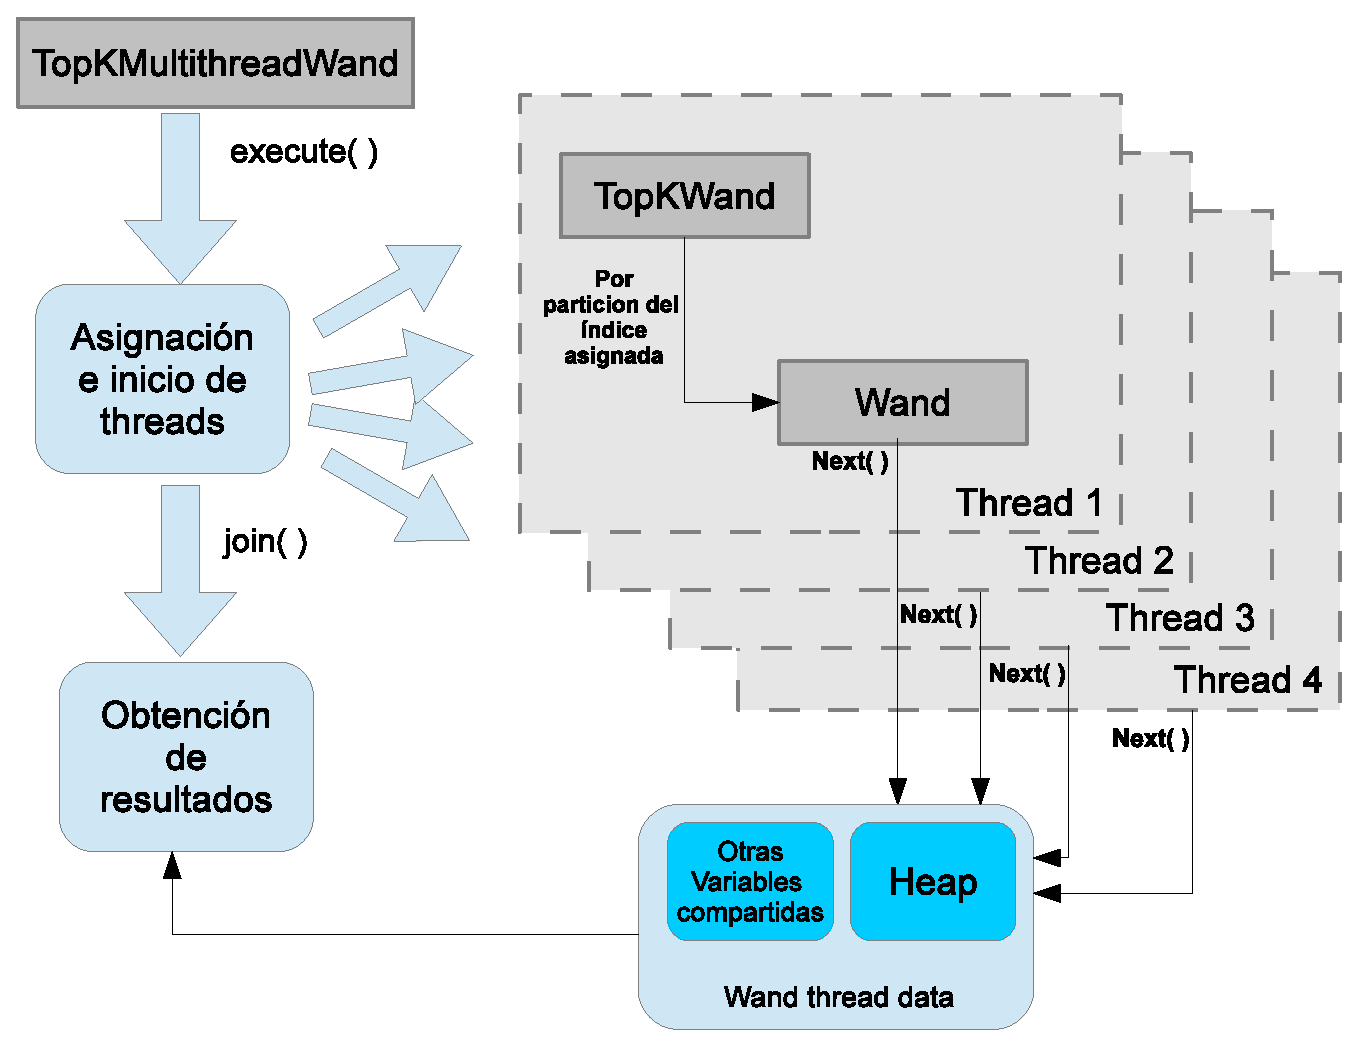
\includegraphics[scale=.75]{images/ejecucion_topkmultithreadwandopCOMPARTIDO.eps}
\caption{Esquema de ejecución enfoque SH}
\label{fig:esquema_ejecucion_wandsh}
\end{figure}












\begin{comment}

// Cómo se llevaron a cabo los experimentos
// Datos
// Máquina
// Programación 


Recordar que en el esquema Wand LH cada uno de los hilos de ejecución computa el conjunto top-K local y luego la hebra maestra hace la mezcla de resultados escogiendo el mejor conjunto top-K global. Este enfoque tiene la ventaja de que es simple de implementar, puesto que no se requiere mecanismos para controlar el paralelismo entre los threads. Sin embargo, se requiere que cada uno de los (P - 1) threads envíe su conjunto solución a la hebra maestra (que también computó su propio conjunto solución), para que crear el resultado final de entre los P x K documentos, donde P es el número de threads encargadas de resolver la consulta y K se es el tamaño del conjunto que se quiere obtener. 

Los resultados en \citep{Rojas:2013} muestran indicios que el esquema LH tendría ventajas por sobre el SH para aquellas transacciones que toman poco tiempo en ser resueltas. 

El Código \ref{code:topkmultithreadwandoperatorlocal} muestra la implementación de la clase que está encargada de llevar a cabo la lógica en la ejecución del enfoque Wand LH. El método execute es el encargado de llegar a cabo la resolución de la consulta, recibe como entrada la query a ser resuelta y un vector de resultados; adicionalmente, este método es el encargado de lanzar los threads con que se resolverá cada consulta y a cada uno de ellos le asiga un objeto de tipo TopKWandOperator (arrops), para obtener los resultados y escribirlos en el vector results. Todo este proceso es llevado a cabo usando el tamaño del conjunto que se quiere obtener (k) y además el índice invertido (indice).


\begin{figure}[!th]
\centering
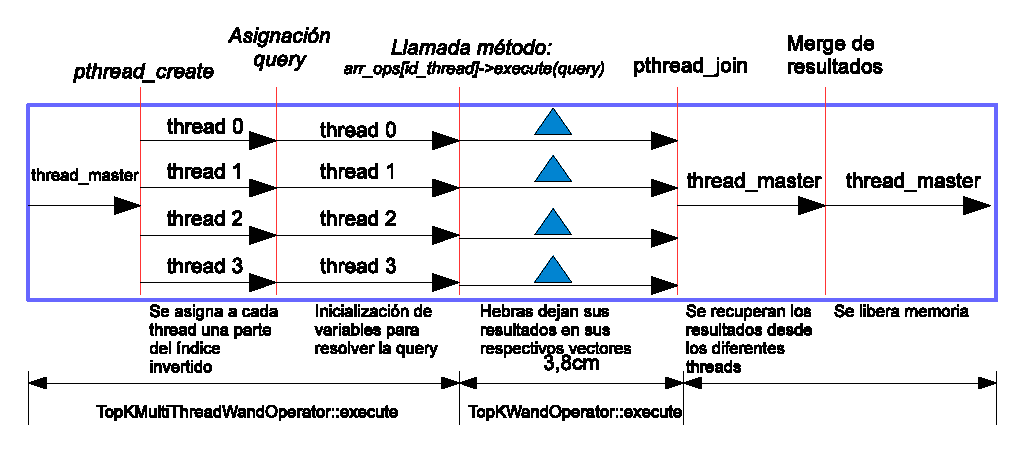
\includegraphics[scale=.75]{images/ejecucion_wandlh.eps}
\caption{Ejemplo de ejecución esquema Wand LH}
\label{fig:ejecucion_wandlh}
\end{figure}

  

%El hecho que en el esquema de heap locales no se requiere mecanismos de control de paralelismo en su implementación, posee ventajas para queries cortas en su procesamiento 
%Figura




\lstinputlisting[label=code:topkmultithreadwandoperatorlocal, caption=Implementación de la clase TopKMultithreadWandOperatorLocal.h, language=C++]{code/TopKMultithreadWandOperatorLocal.h}

Mostrar topK Wand operator

\end{comment}



\begin{comment}

el proceso de descarte tiende a ser más eficiente porque los documentos con mayor puntaje tienden a estar en el heap

Se habla un poco de las ventajas que se tenía con este esquema nuevamente, qué se hizo para la implementación, cómo se programó, etc. 

Se muestra el código y ojalá se muestra algún flujo de ejecución para una query específica.

%\lstinputlisting[language=C++]{code/TopKMultithreadWandOperatorLocal.h}

Se muestra un gráfico y tabla de eficiencia.

\end{comment}

\subsection{Resultados obtenidos}
\label{evaluacionexperimental:resultadosObtenidos}

En la Figura \ref{fig:tiempos_wand} se puede observar el tiempo promedio del enfoque LH y el enfoque SH en resolver un conjunto de 10000 consultas de la colección gov2. A medida que crece el número de threads, el enfoque de heaps compartidos toma ventaja por sobre el enfoque de heaps locales, sin embargo, con un thread se puede observar que LH (117.486 ms) requiere un tiempo menor que SH (130.591 ms), esto se debe porque aquí no se usa una estructura de dato compartida que retrase a los hilos de ejecución esperando a que otros la liberen. LH requiere menos tiempo en resolver el log de consultas para 2,4,8 y 16 threads. 

El esquema LH puede estar muy supeditado a la distribución de documentos en las listas del índice invertido, ya que si un thread procesa su parte corrrespondiente del índice invertido en donde los mejores puntajes se encuentran al final, entonces el heap tendrá un umbral bajo el proceso de descarte omitirá pocos documentos, esto implca que el tiempo de ejecución requerido será mayor, retrasando el proceso que mezcla los resultados para obtener el conjunto top-K dinal. 

Como el esquema SH ocupa un solo heap para obtener el conjunto top-K final, el heap tiende a llenarse rápidamente con los mejores documentos globales, esto implica que el puntaje mínimo del heap (que trabaja de umbral) tiende a crecer rápidamente, permitiendo un mejor descarte de documentos y menos tiempo de ejecución para las hebras. 

Adicionalmente en la Figura \ref{fig:eficiencias_wand} se puede ver que en forma general con la estrategia de enfoques compartidos se obtiene mejores eficiencias que con la estrategia LH. En Con SH la mejor eficiencia que se obtiene es con 4 threads (0.962 ms), mientras que con 2 y con 8 threads se obtiene una eficiencia de 0.887 y 0.8312600071 milisegundos; en general se obtiene buenas eficiencias para 1,2,4 y 8 hebras, sin embargo, con 16 threads la eficiencia baja considerablemente (0.5403329185) con respecto a las anteriores, esto se debe principalmente a la tecnología hyperthreading de la máquina utilizada y que el uso exclusivo del heap compartido por parte de los threads no tiene un fuerte impacto en el rendimiento.  
La eficiencia baja de LH se debe porque para obtener el conjunto top-K final de una consulta debe haber una sincronización de todos los threads en que cada uno de ellos envíe sus top-K locales a la hebra maestra y además porque existe un costo adicional de calcular el conjunto top-K final entre los P * K documentos seleccionados (siendo P el número de procesadores). 
                     
Para los siguientes experimentos del presente trabajo se ocupará el enfoque SH para resolver las transacciones de lectura.


\begin{figure}[!ht]
\centering
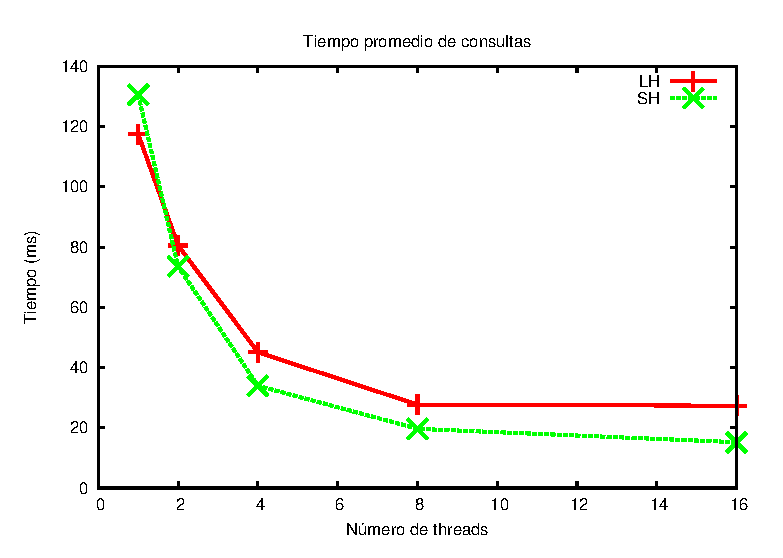
\includegraphics[scale=.75]{images/tiempos_wand.eps}
\caption{Tiempos promedios de las consultas}
\label{fig:tiempos_wand}
\end{figure}

\begin{figure}[!ht]
\centering
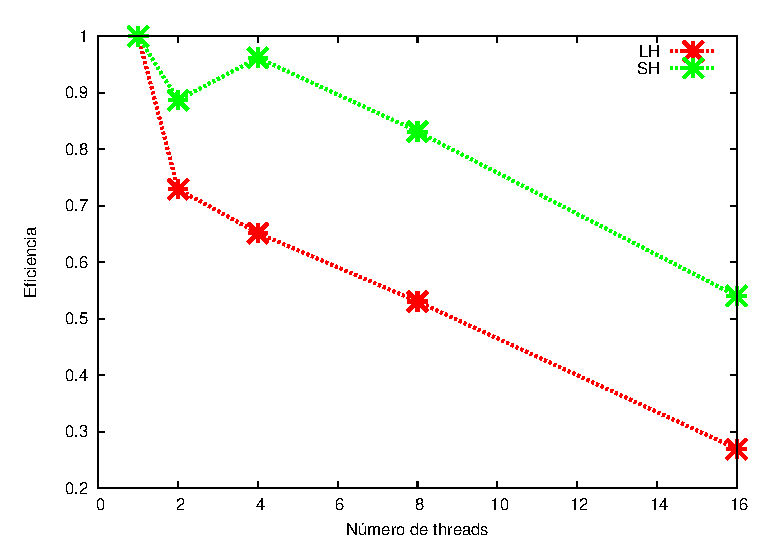
\includegraphics[scale=.75]{images/eficiencias_wand.eps}
\caption{Eficiencias para Wand con heaps compartido y locales}
\label{fig:eficiencias_wand}
\end{figure}


\begin{comment}

Se hace una introducción.

\section{Predicción de tiempo de respuesta a transacción de lectura}
\label{evaluacionexperimental:ptrq}
Se hace experimentos con predictor perfecto

Nosotros optamos por un enfoque de Wand Heap Compartido para ser usado en los experimentos.

Se hace una breve introducción al cpaítulo anterior. 

Se menciona los resultados obtenidos con la regresión, se dice que no se tuvieron muy buenos resultados con la regresión, se deja a ver por qué no se obtuvieron muy buenos resultados (índice con los que se hicieron experimentos, consultas, etc.).

	//menos que 10% tpo esperado, menos que 25%, menos que 50% y el resto (en el timesRanges)
\subsection{Predictor perfecto}
\label{evaluacionexperimental:predictorperfecto}

Decir que no es el foco de esta tesi, que los resultados obtenidos no fueron muy buenos s y que para evaluar los algoritmos de scheduling  también se usará un predictor perfecto. Decir cómo se obtuvo un predictor perfecto y ojalá mostrar algún algoritmo.





\section{Estrategias de scheduling}
\label{evaluacionexperimental:estrategiasscheduling}

Hablar separado cada una de ellas, mostrando implementación y cómo se llevaron a cabo los experimentos.

1. Comparar las tres estrategias de scheduling (decir que TimesRanges es mejor) ==> Con predictor perfecto también?
2. Comparar TimesRanges con baseline ==> Con Predictor perfecto también.  
4. Decir los problemas que existen en cada una de las estrategias que se pierden tiempos.
3. Sacar a la luz la nueva unidades de trabajo ==> Predictor perfecto también.
4. Comparación unidades de trabajo - baseline - TimesRanges.

Conclusiones para cada uno de los gráficos realizados. 

Se intuye que habrá pérdida de eficiencia al final de cada bloque en FR.

\end{comment}